\documentclass{beamer}

\mode<presentation>
{%
  \usetheme[alternativetitlepage=bild]{Rub}
  \titlegraphic{img-bg.jpg}
  \sponsorlogo[height=15mm]{img-gdata.pdf}

  \setbeamercovered{transparent}
}
\usepackage{rubfonts2009}
\usepackage[english]{babel}
\usepackage[utf8]{inputenc}
\usepackage[babel,english=american]{csquotes}
\usepackage{mathptmx}
\usepackage[scaled=.90]{helvet}
\usepackage{courier}
\usepackage{amsmath}
\usepackage{protocol}

\usepackage[T1]{fontenc}

\title{Hack.Lu 2013 Challenges}
\subtitle{ECKA, Geiers Lambda, Marvin is plane-Jane}
\author{Friedrich~Wiemer}
\institute[Ruhr Universit\"at Bochum]
{%
  FluxFingers\\
  Ruhr Universit\"at Bochum
}

\date{12. Februar 2014}

\subject{Theoretical Computer Science}

% Delete this, if you do not want the table of contents to pop up at
% the beginning of each subsection:
\AtBeginSection[]
%{%
%  \begin{frame}<beamer>{Outline}
%    \tableofcontents[currentsection,currentsubsection]
%  \end{frame}
%}

% If you wish to uncover everything in a step-wise fashion, uncomment
% the following command:

%\beamerdefaultoverlayspecification{<+->}

\begin{document}

\begin{frame}
    \titlepage{}
\end{frame}

\begin{frame}{Outline}
  \tableofcontents
  % You might wish to add the option [pausesections]
\end{frame}

\section{ECKA}
\begin{frame}{ECKA}
    \begin{figure}[!htb]
        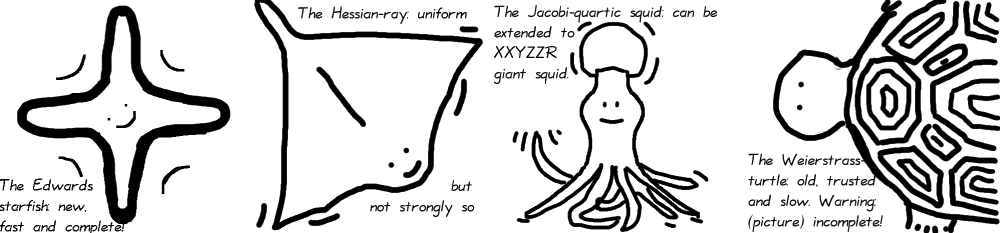
\includegraphics[height=25mm]{data/ec-types.png}
    \end{figure}
    \begin{figure}[!htb]
        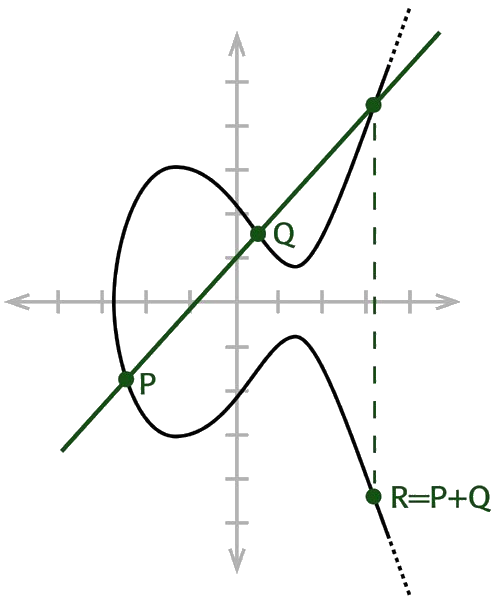
\includegraphics[height=25mm]{data/ec.png}\hspace{10mm}
        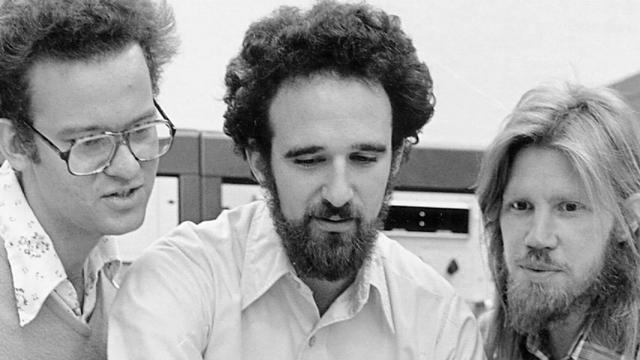
\includegraphics[height=25mm]{data/merkle-hellman-diffie.jpg}\hspace{10mm}
        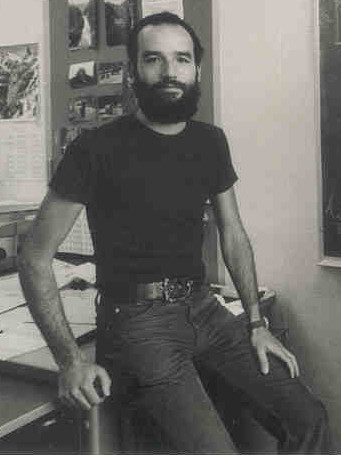
\includegraphics[height=25mm]{data/shamir.jpg}
    \end{figure}
\end{frame}

\subsection{Challenge}
\begin{frame}{Story}{Infos}
    \begin{itemize}
        \item Service using key agreement on elliptic curves
        \item Combines two different ones: \begin{enumerate}
           \item Exchange a point P
           \item Agree on key
           \item Send AES-ECB encrypted password
        \end{enumerate}
    \end{itemize}
    Hint: He, we have the latest news for you.
    The first part of their strange key agreement
    was designed by the famous SHA-Robot \textsc{Mir}!
\end{frame}

\begin{frame}{Stats}
    \begin{itemize}
        \item Category: Crypto
        \item Points: 100
        \item Solved by: 5 Teams
    \end{itemize}
\end{frame}

\subsection{Service}
\begin{frame}{Service}
    \begin{figure}[!htb]
        
\includegraphics[height=45mm]{data/demo.png}
    \end{figure}
\end{frame}

\subsection{Crypto Stuff}
\begin{frame}{Crypto Stuff}
    Involved Crypto-Stuff
    \begin{itemize}
        \item Elliptic Curve Crypto (ECC)
        \item Key Agreements: \begin{itemize}
            \item ThreePass
            \item Diffie Hellman
        \end{itemize}
    \end{itemize}
\end{frame}
\begin{frame}{ECC}{Elliptic Curve Cryptography}
    \begin{itemize}
        \item asymmetric crypto
        \item uses elliptic curves over finite fields as group
        \item thus can replace other groups (normally $\mathbb{Z}_p^*$)
        \item good properties like small key size etc.
    \end{itemize}
    \begin{itemize}
        \item Discrete Logarithm Problem (DLP) is hard
        \item algorithms like DHKE, Elgamal can be used
    \end{itemize}
\end{frame}

\begin{frame}{ThreePass}{on Elliptic Curves}
\begin{figure}[!htb]
    \begin{protocol}{2}
    \protocolheader{$\mathcal{E}(\mathbb{Z}_p^*)$}
    \participants{\textbf{Alice}}{\textbf{Bob}}\\ 
        \doesA{$\alpha \in_R \mathbb{Z}_p^*$}
        \doesA{$P \in \mathcal{E}(\mathbb{Z}_p^*)$}
        \doesA{$P_{\alpha} = \alpha P$}
        & \sends{P_{\alpha}} & \\[-5mm]
        \doesB{$\beta \in_R \mathbb{Z}_p^*$}
        \doesB{$P_{\alpha\beta} = \beta P_{\alpha}$}
        &\receives{P_{\alpha\beta}} & \\[-5mm]
        \doesA{$P_{\beta}=\alpha^{-1}\cdot P_{\alpha\beta}$}
        & \sends{P_{\beta}} & \\[-5mm]
        \doesB{$P=\beta^{-1}\cdot P_{\beta}$}
    \end{protocol}
\end{figure}
\end{frame}

\begin{frame}{DHKE}{on Elliptic Curves}
\begin{figure}[!htb]
    \begin{protocol}{2}
    \protocolheader{$\mathcal{E}(\mathbb{Z}_p^*),\,P \in \mathcal{E}(\mathbb{Z}_p^*)$}
    \participants{\textbf{Alice}}{\textbf{Bob}}\\ 
        \doesA{$\alpha \in_R \mathbb{Z}_p^*$}
        \doesA{$P_{\alpha} = \alpha P$}
        & \sends{P_{\alpha}} & \\[-5mm]
        \doesB{$\beta \in_R \mathbb{Z}_p^*$}
        \doesB{$P_{\beta} = \beta P$}
        &\receives{P_{\beta}} & \\[-5mm]
        \doesA{$P_{\alpha \beta}=\alpha \cdot P_{\beta}$}
        \doesB{$P_{\alpha \beta}=\beta \cdot P_{\alpha}$}
    \end{protocol}
\end{figure}
\end{frame}

\subsection{Solution}
\begin{frame}{Solution}
    \begin{figure}[!htb]
        
\includegraphics[height=45mm]{data/demo.png}
    \end{figure}
\end{frame}

\section{Geiers Lambda}
\begin{frame}{Geiers Lambda}
    \begin{figure}[!htb]
        
\includegraphics[height=35mm]{data/eagle.png}\hspace{10mm}
        
\includegraphics[height=35mm]{data/haskell.png}
    \end{figure}
\end{frame}

\subsection{Challenge}
\begin{frame}{Story}{Infos}
    Given:
    \begin{itemize}
        \item encrypted defusing-password
        \item haskell code for decryption
        \item collision for decryption password
    \end{itemize}

    Infos:
    \begin{itemize}
        \item decryption password consists of 8 alphanumeric chars
        \item defusing password contains only printable characters
    \end{itemize}
\end{frame}

\begin{frame}{Stats}
    \begin{itemize}
        \item Category: Crypto
        \item Points: 200
        \item Solved by: 16 Teams
    \end{itemize}
\end{frame}

\subsection{Haskell Code}
\begin{frame}{Haskell Code}
    \visible<2->{%
    \begin{itemize}
        \item used almost only lambda (anonymous) functions
        \item two interesting functions: \textsc{hash} and \textsc{dec}
        \item magic constant in \textsc{dec} $\Rightarrow$ \textsc{TEA}
        \item \textsc{hash} seems to be adler32
    \end{itemize}
    }
    
    \visible<3->{Collision Finding:
    \begin{itemize}
        \item $\text{Byte}[n] + k$
        \item $\text{Byte}[n+1] - 2k$
        \item $\text{Byte}[n+2] + k$
    \end{itemize}
    }
\end{frame}

\subsection{Solution}
\begin{frame}{Solution}
    \begin{figure}[!htb]
        
\includegraphics[height=45mm]{data/demo.png}
    \end{figure}
\end{frame}

%\section{Marvin is plane-Jane}
\begin{frame}{Marvin is plane-Jane}
    \begin{figure}[!htb]
        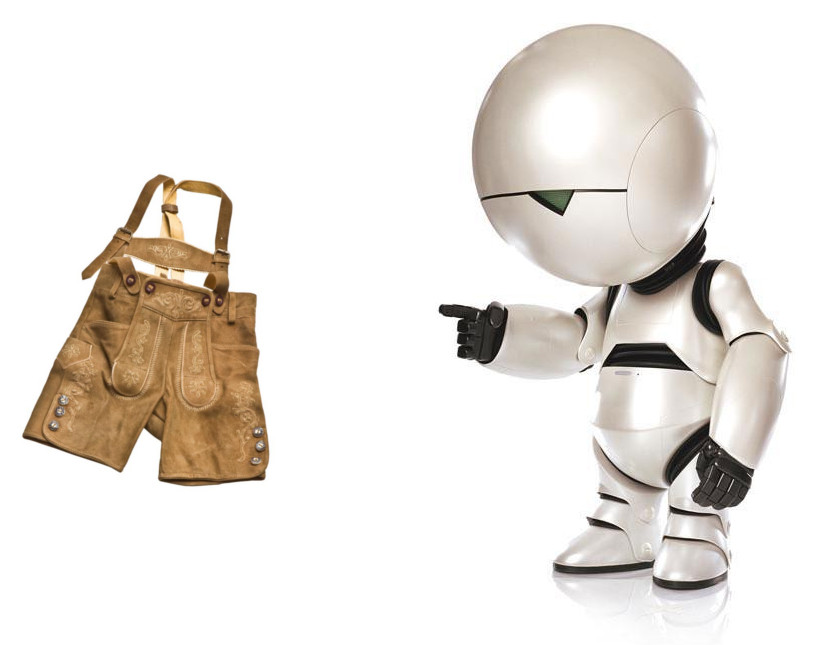
\includegraphics[height=60mm]{data/marvin.jpg}
    \end{figure}
\end{frame}

\subsection{Challenge}
\begin{frame}{Story}{Infos}
    \begin{itemize}
        \item \emph{Marvin is}
        \item using brainpool p256r1
        \item his friend is called meneze or something --- or was it van-stone?\\[5mm]
        \item $(23372093078317\ldots7754827452856 : 1)$
        \item $711644502408974\ldots8605658194656$
        \item $129516935171006\ldots4560064909824$\\[5mm]
        \item Find out what \emph{Marvin is}
    \end{itemize}
\end{frame}

\begin{frame}{Stats}
    \begin{itemize}
        \item Category: Crypto
        \item Points: 100
        \item Solved by: 3 Teams
    \end{itemize}
\end{frame}

\subsection{Crypto Stuff}
\begin{frame}{Crypto Stuff}{Menezes-Vanstone Cipher}
    \begin{itemize}
        \item Global Parameter: $\mathcal{E}(\mathbb{Z}_p^*)$
        \item Public-Key: $P, Q \in \mathcal{E}(\mathbb{Z}_p^*)$
        \item Secret-Key: $\alpha \in \mathbb{Z}_p^*$, s.t. $Q = \alpha \cdot P$
    \end{itemize}
\end{frame}

\begin{frame}{Crypto Stuff}{Menezes-Vanstone Cipher}
    Enc:
    \begin{itemize}
        \item message $m = (m_1,m_2) \in \mathbb{Z}_p^* \times \mathbb{Z}_p^*$
        \item randomization $r \in_R \mathbb{Z}_p^*$\\
        \item compute:
            \begin{itemize}
                \item $(b_1,b_2) = r \cdot Q$
                \item $R = r \cdot P$
                \item $c_1 = b_1 \cdot m_1 \bmod p$
                \item $c_2 = b_2 \cdot m_2 \bmod p$
            \end{itemize}
        \item output ciphertext $c = (R, c_1, c_2)$
    \end{itemize}
\end{frame}

\begin{frame}{Crypto Stuff}{Menezes-Vanstone Cipher}
    Dec:
    \begin{itemize}
        \item ciphertext $c = (R, c_1, c_2) \in \mathcal{E}(\mathbb{Z}_p^*) \times \mathbb{Z}_p^* \times \mathbb{Z}_p^*$
        \item compute:
            \begin{itemize}
                \item $\alpha \cdot R = \alpha \cdot r \cdot P = r \cdot Q = (b_1,b_2)$
                \item $m_1 = b_1 \cdot c_1^{-1} \bmod p$
                \item $m_2 = b_2 \cdot c_2^{-1} \bmod p$
            \end{itemize}
        \item output message $m = (m_1, m_2)$
    \end{itemize}
    Note:
    \begin{itemize}
        \item knowledge of $r \cdot Q$ is needed for decryption
        \item computing of $r \cdot Q$ looks as hard as solving\\
              $r = \text{dlog}_Q(R)$ or \\
              $\alpha = \text{dlog}_P(Q)$
    \end{itemize}

\end{frame}

\begin{frame}{Crypto Stuff}{Menezes-Vanstone Cipher}
    Correctness:
    \visible<2->{%
    \begin{itemize}
        \item Just kidding :) \\[2cm]
    \end{itemize}
    }

    \visible<3->{%
    But where are the flaws?
    }
\end{frame}

\begin{frame}{Crypto Stuff}{Menezes-Vanstone Cipher}
    Observation:
    \begin{itemize}
    \visible<1->{%
        \item $c = (R, c_1, c_2)$, s.t. \\
              $c_1 = b_1 \cdot m_1 \bmod p$ and $c_2 = b_2 \cdot m_2 \bmod p$
              \begin{align*}
                  c_1 = b_1 \cdot m_1 \bmod p &&\Rightarrow&& c_1 \cdot m_1^{-1} = b_1 \bmod p
              \end{align*}
        \item $b_1$ is the x coordinate of $r \cdot Q$
    }
    \visible<2->{%
        \item there are only two points on $\mathcal{E}(\mathbb{Z}_p^*)$ with $b_1$ as their x coordinate
        \item trying both give us two possibilities for $r \cdot Q$
    }
    \visible<3->{%
        \item two possibilities for message without computing a discrete log
    }
    \end{itemize}
    \visible<4->{%
    What do we need for this?
    \begin{itemize}
        \item $c_1 \cdot m_1^{-1} = b_1 \bmod p$\\
              $\Rightarrow$ $(c_1, m_1)$, first half of a plaintext/ciphertext pair
    \end{itemize}
    }
\end{frame}

\subsection{Solution}
\begin{frame}{Solution}
    \begin{figure}[!htb]
        
\includegraphics[height=45mm]{data/demo.png}
    \end{figure}
\end{frame}


\section*{Summary}
\begin{frame}{Appendix}
    Challenges
    \begin{small} \begin{itemize}
        \item \url{https://ctf.fluxfingers.net/2013/challenges/1}
        \item \url{https://ctf.fluxfingers.net/2013/challenges/2}
%        \item \url{https://ctf.fluxfingers.net/2013/challenges/3}
    \end{itemize} \end{small}

    Write-Ups
    \begin{small} \begin{itemize}
        \item \url{https://stratum0.org/blog/blog/2013/10/26/hack-dot-lu-2013-ecka/}
        \item \url{http://balidani.blogspot.pt/2013/10/hacklu-ctf-crypto-200-geiers-lambda.html}
%        \item \url{https://stratum0.org/blog/blog/2013/10/26/hack-dot-lu-2013-marvin-is-plain-jane/}
    \end{itemize} \end{small}
\end{frame}

\begin{frame}{Questions?}{Thanks!}
    \begin{figure}[!htb]
        
\includegraphics[height=50mm]{data/questions.png}
    \end{figure}
\end{frame}

\end{document}
